\chapter{Basics}

Little-$o()$ notation is used to denote that some expression is small relative to some other value.

\begin{marginfigure}
\includegraphics[width=0.75\linewidth]{graphics/basics1.pdf}
\caption[$(1 + h )^3 = 1 + 3 h + o(h)$ as $h \rightarrow 0$.]{$(1 + h )^3 = 1 + 3 h + o(h)$ as $h \rightarrow 0$.  Notice how the curves are {\em tangent} (touch and align) at $h=0$.}
\label{fig:basics1}
\end{marginfigure}
For example, if we say:
\begin{equation*}
(1 + h)^3 = 1 + 3 h + o(h)\text{\ as\ }h \rightarrow 0\,.
\end{equation*}
We mean that, as the magnitude of $h$ gets smaller, the magnitude of the difference between the left-hand side  $L = (1 + h )^3$ and the  right-hand side $R = 1 + 3 h$  is so small that, even when divided by $h$,  it is still small.  

We can check this ratio empirically: 
\begin{table}
\caption{$(1 + h )^3 = 1 + 3 h + o(h)$ as $h \rightarrow 0$.}
\label{tab:basic1}
\begin{tabular}{|S[table-format=2.3]|S[table-format=2.9]|S[table-format=2.3]|S[table-format=2.11]|S[table-format=2.6]|}
\multicolumn{1}{c}{$h$} & 
\multicolumn{1}{c}{$L=(1+h)^3$} & 
\multicolumn{1}{c}{$R=1+3h$} & 
\multicolumn{1}{c}{$E=L-R$} &
\multicolumn{1}{c}{$r=\left|\frac{E}{h}\right|$} \\
\hline
0.1  & 1.331 & 1.3 & 0.031 & 0.31 \\
\hline
-0.01 & 0.970299 & 0.97 & 0.000299 & 0.0299 \\
\hline
0.001 & 1.003003001 & 1.003 & 0.00000030001 & 0.003001 \\
\hline
\end{tabular}
\end{table}

Notice how the ratio  $r=|E/h|$ shrinks as the magnitude of $h$ shrinks.  When we say an expression  $E$  is $o(h)$ as  $h \rightarrow 0$,  we mean the magnitude of $|E/h|$  gets small as the magnitude of $h$ gets small.

Graphically, smooth expressions that differ by $o(h)$ are {\em tangent} (touch and align) at $h=0$.  This is illustrated for this example in figure~\ref{fig:basics1}.

\begin{marginfigure}
\includegraphics[width=0.75\linewidth]{graphics/basics2.pdf}
\caption{$2k^3+5k^2-7k+3=2k^3+o(k^3)$ as $k \rightarrow \infty$.  Note how similar the curves are for large magnitude $k$.}
\label{fig:basics2}
\end{marginfigure}
\begin{marginfigure}
\includegraphics[width=0.75\linewidth]{graphics/basics3.pdf}
\caption{$2k^3+5k^2-7k+3=2k^3+o(k^3)$ as $k \rightarrow \infty$.  Note how dissimilar the curves are for small magnitude $k$.}
\label{fig:basics3}
\end{marginfigure}
The  $o()$  notation allows for more general expressions for the relative comparison of smallness,  such as  $o(h^2)$ or  $o(h \ln(h))$. In each case, we are saying that the expression in question is small in magnitude when divided by the expression in the $o()$  as the parameter ($h$ in this case) gets small in magnitude.

The notation works for large parameters as well.  For example: 
\begin{equation}
2k^3 + 5 k^2 - 7 k + 3 = 2k^3 + o (k^3 )\text{\ as\ }k \rightarrow \infty \,.
\end{equation}
This means, as the magnitude of  $k$ gets larger and larger, the cubic polynomial on the left is approximately the leading order term (term with the highest power of  $k$) plus an error small relative to the size of that term.   Comparing figure~\ref{fig:basics2} and figure~\ref{fig:basics3} illustrates this trend, and table~\ref{tab:basics2} gives example values as $k \rightarrow \infty$.

\begin{table}
\caption[$2k^3 + 5 k^2 - 7 k + 3=2k^3+o(k^3)$]{$2k^3 + 5 k^2 - 7 k + 3=2k^3+o(k^3)$.  Notice how the error $E$ grows, but it is still small when compared to $\varepsilon(k) = k^3$.}
\label{tab:basics2}
\begin{tabular}{|S[table-format=4]|S[table-format=10]|S[table-format=10]|S[table-format=7]|S[table-format=10]|S[table-format=1.5]|}
\multicolumn{6}{c}{\vspace{2em}} \\
\multicolumn{1}{l}{$k$} & 
\multicolumn{1}{l}{$\begin{array}{c}L=2k^3+ 5 k^2 \\ - 7 k + 3\end{array}$} &\multicolumn{1}{l}{$R=2k^3$} & 
\multicolumn{1}{l}{$E=L-R$} &
\multicolumn{1}{l}{$\varepsilon(k)=k^3$} &
\multicolumn{1}{l}{$r=\left|\frac{E}{\varepsilon(k)}\right| $} \\
\hline
10  & 2433 & 2000 & 433 & 1000 & 0.43300 \\
-100 & -1949297 &  -2000000 & 50703 & -1000000 & 0.05070 \\
1000 & 2004993003 & 2000000000 & 4993003 & 1000000000 & 0.00499 \\
\hline
\end{tabular}
\end{table}

\section{Euler's constant, $e$.}
Euler's constant $e \approx \num{2.718281828459045}$ is fundamental for exponents and logarithms, just as  $\pi \approx \num{3.141592653589793} $ is fundamental in trigonometry.  

The value $e$ can be thought of as the value of the expression $(1 + h)^{1/h}$ as $h \rightarrow 0$.  In $o()$ notation\footnote{Writing $1$ as  $h^0$ in $o(h^0)$ may seem surprising, but it is a way of noting what parameter is getting small.}: 

\begin{equation}
(1 + h)^{1/h}=e+o(h^0)\text{\ as\ } h \rightarrow 0\,.
\end{equation}

This means, as the magnitude of  $h$ gets smaller and smaller, the expression on the left is approximately $e$, plus an error small relative to $h^0=1$.  Figure~\ref{fig:e} and table~\ref{tab:e} demonstrate this.  Notice $(1 + h )^{1/h}$ is not defined for $h=0$, but we only care about small {\em nonzero} values of $h$.

Curves that differ by $o(h^0)$ need only try to touch at $h=0$ (unlike $o(h)$ errors, where they need to be tangent).
 
\begin{table}
\caption{$(1 + h )^{1/h}=e+o(h^0)$.}
\label{tab:e}
\begin{tabular}{|S[table-format=2.6]|S[table-format=2.9]|S[table-format=1.8]|}
\multicolumn{1}{c}{$h$} & 
\multicolumn{1}{c}{$(1+h)^{1/h}$} &
\multicolumn{1}{c}{$r=\left|\frac{(1+h)^{1/h}-e}{1}\right| $} \\
\hline
0.01 & 2.704813829 & 0.0135 \\
-0.0001 & 2.718417755 & 0.000136 \\
0.000001 & 2.718280469 & 0.00000136 \\
\hline
\end{tabular}
\end{table}
\vspace{4em}
\begin{marginfigure}
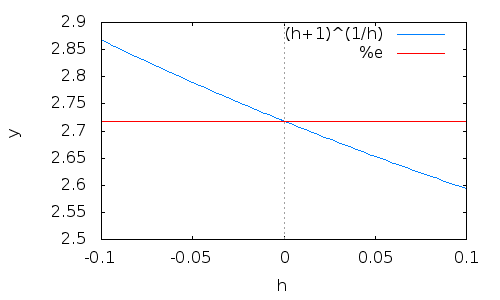
\includegraphics{graphics/e.pdf}
\caption[$(1 + h )^{1/h}=e+o(h^0)$]{$(1 + h )^{1/h}=e+o(h^0)$.  Notice the curves only try to touch (instead of be tangent) at $h=0$.}
\label{fig:e}
\end{marginfigure}
   
\section{Sine.}
As $h \rightarrow 0$,  $\sin(x+h)=\sin(x)+\cos(x)h + o(h)$.    
\begin{marginfigure}
\includegraphics{graphics/sine.pdf}
\caption{$\sin(x+h)=\sin(x)+\cos(x) h+o(h)$ for $x=1$ and $\pi$.}
\label{fig:sine}
\end{marginfigure}
 
We will show this is true later, but, geometrically, it means that evaluating  $y=\sin(x)$ near $x$ is approximately a line\footnote{A line going through the point $(x_0,y_0)$ with slope $m$ is $y=y_0+m \cdot (x-x_0)$.} going through the point  $(x,\sin(x))$ with slope  $\cos(x)$. 

\begin{figure}
\includegraphics{graphics/calc.pdf}
\caption[Differential calculus.]{Differential calculus in a nutshell: often, the value of $f(x)$ near $x$ is approximately a line: $f(x+h)=f(x)+f'(x)h+o(h)\,$.}
\label{fig:calc}
\end{figure}
{\em This last example is really important.}  The idea that, near a given point  $x$,  many functions are well approximated by a line is a foundational idea of differential calculus.  We call such a function differentiable at $x$, and the slope of its tangent line  $f'(x)$, so that $f(x+h)=f(x)+f'(x)h+o(h)$.  For the example of figure~\ref{fig:sine}, we are saying that, if $f(x) = \sin(x)$, then  $f'(x)=\cos(x)$.  

\marginnote{Always writing ``as  $h \rightarrow 0$'' is tedious.  It will be clear from the $o()$ notation which parameter we consider large or small.}

In general, $o(h^0)$ approximations touch at $h=0$, $o(h^1)$ approximations have the same tangent (best fitting line), and $o(h^2)$ approximations have the same curvature (best fitting circle).  Figure~\ref{fig:rates} illustrates this with approximations of $e^h$.
\begin{figure}
\begin{center}
\includegraphics[width=4in]{graphics/rates.pdf}
\end{center}
\caption[Comparing $o(h^p)$]{Three progressively better approximations of $e^h$ as $h \rightarrow 0$: 

$e^h=1+o(h^0)$, 

$e^h=1+h+o(h^1)$, and 

$e^h=1+h+\frac{h^2}{2}+o(h^2)$. 

Notice the $o(h^0)=o(1)$ approximation touches, the $o(h^1)=o(h)$ approximation is tangent (best fitting line), and the $o(h^2)$ approximation has the same curvature (best fitting circle) at $h=0$.}
\label{fig:rates}
\end{figure}

\section{Formalities}
\begin{figure}
\begin{center}
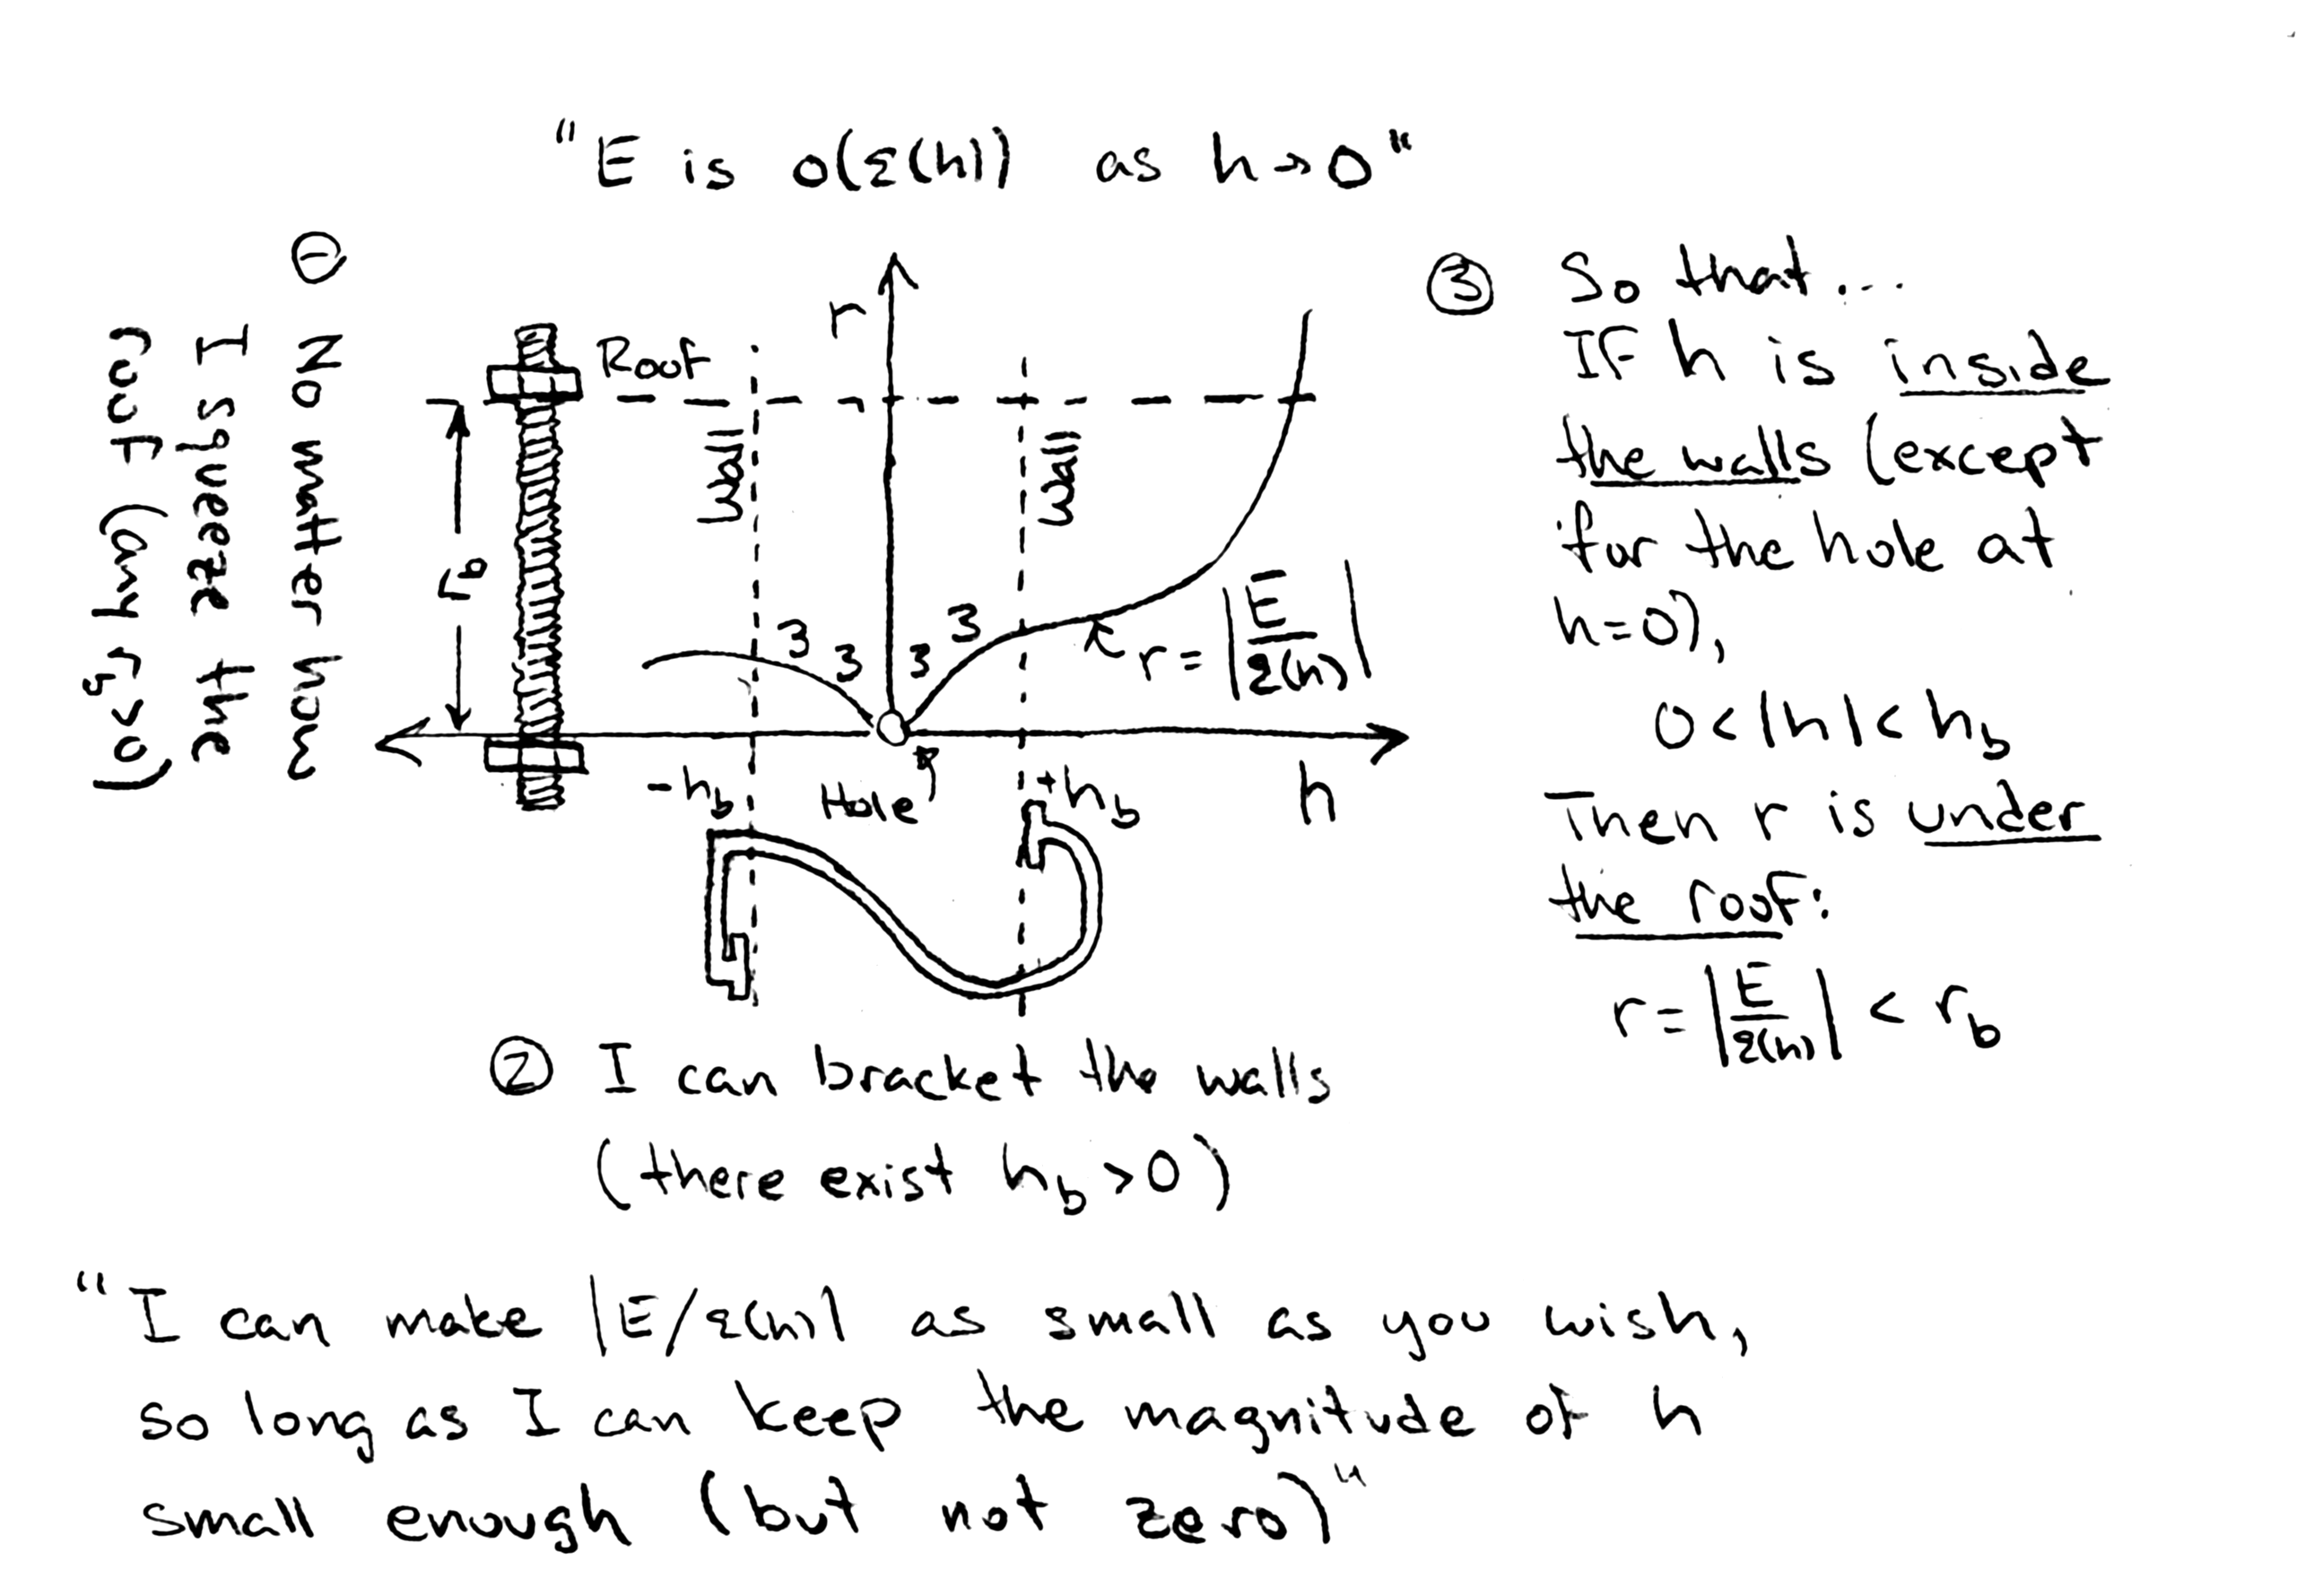
\includegraphics[width=4in]{graphics/littleo.png}
\end{center}
\caption[$o()$ sketch.]{Sketch of the meaning of $o()$.  Redraw this in your notes so you remember the definition of little-$o()$.}
\label{fig:littleo}
\end{figure}

An expression $E$ is  $o(\varepsilon(h))$ as $h \rightarrow 0$ when the ratio $r = \left| \frac{E}{\varepsilon(h)} \right|$ is smaller than any positive bound $r_b$, provided we force the magnitude of $h$ to be small enough (but not zero). 

Specifically\footnote{If you are familiar with limit notation, $E$ is  $o(\varepsilon(h))$ as $h \rightarrow 0$ means $\lim_{h\rightarrow 0} \left|\frac{E}{\varepsilon(h)}\right| = 0$.} $E$ is  $o(\varepsilon(h))$ if, and only if, for any bound $r_b>0$, there exists a bound $h_b>0$, so that $r=|E/\varepsilon(h)|<r_b$ whenever $0 < |h| < h_b$.

We define\footnote{If you are familiar with limit notation, $E$ is  $o(\varepsilon(k))$ as $k \rightarrow \infty$ means $\lim_{k\rightarrow \infty} \left|\frac{E}{\varepsilon(k)}\right| = 0$.} large $k$ in terms of small $h$ by saying $E$ is $o(\varepsilon(k))$ as $k \rightarrow \infty$ means $E$ is $o(\varepsilon(1/h)$ as $h \rightarrow 0$.  In other words, for any bound $r_b>0$, there exists a bound $k_b>0$, so that $r=|E/\varepsilon(h)|<r_b$ whenever $|k|>k_b$.
 
Note that we divide $E$ by $\varepsilon(h)$ to get $r$  in the above definition for some range of nonzero values of $h$. So, for any expression to be $o(\varepsilon(h))$,  $\varepsilon(h)$  must be defined and nonzero for some range of nonzero values of $h$.  We therefore restrict $\varepsilon(h)$ to such admissible functions:   

\begin{quote}
For $\varepsilon(h)$ to be admissible in $o(\varepsilon(h))$ notation, there must exist some  $h_0 > 0$ so that $\varepsilon(h)$ is defined (finite) and nonzero for  $0 < |h| < h_0$.  This way we can form the ratio $r=|E/\varepsilon(h)|$ without dividing by zero for at least some range of $h$.
\end{quote}
 
We only use admissible $\varepsilon(h)$ in these notes.  In particular, $\varepsilon(h) = {|h|}^p$  is admissible for any value of  $p$ , and $\varepsilon(h) = h^p$ is admissible for any integer value of $p$.  

\section{Summary}
\begin{itemize}
\item
Little-$o()$ notation is a way of describing an expression as small in comparison to some other value: 
\begin{quote}
  $E$ is $o(\varepsilon(h))$ as $h \rightarrow 0$ means the ratio  $r = |E/\varepsilon(h)|$  can be made as small as desired provided the magnitude of $h$ is small enough (but not zero).
\end{quote}

\item 
Graphically, expressions that differ by $o(h^0)$ need to touch at $h=0$, but expressions that differ by $o(h^1)$ also need to be tangent at $h=0$.

\item
Specifically,  $E$ is $o(\varepsilon(h))$  as $h \rightarrow 0$  means:  
\begin{quote} 
For any  $r_b > 0$,  there exists $h_b > 0$,  so that:
\begin{equation*}
\text{if\ } 0 < | h | < h_b\,,\text{\ then\ }r=\left|\frac{E}{\varepsilon(h)}\right|<r_b\,.
\end{equation*}
\end{quote}

\item 
$E$ is $o(\varepsilon(k))$ as $k \rightarrow \infty$ means
\begin{quote}
$E$ is $o(\varepsilon(1/h)$ as $h \rightarrow 0$.
\end{quote}
or
\begin{quote} 
For any  $r_b > 0$,  there exists $k_b > 0$,  so that:
\begin{equation*}
\text{if\ } |k| > k_b\,,\text{\ then\ }r=\left|\frac{E}{\varepsilon(h)}\right|<r_b\,.
\end{equation*}
\end{quote}

\item 
For differentiable functions, the value $f(x+h)$ near a given point $x$ is well  approximated by a line called the tangent line of $y=f(x)$  at $x$ with slope $f'(x)$.

\item ${(1+h)}^{(1/h)} = e + o(h^0)$ as $h \rightarrow 0$,  where  $e \approx 2.718$ is Euler's constant.

\item Because an expression $E$ is divided by $\varepsilon(h)$ in the definition of $o(\varepsilon(h))$, $\varepsilon(h)$  is admissible in $o(\varepsilon(h))$ notation only if it is defined and nonzero for small enough nonzero $h$.
\begin{quote}
For $\varepsilon(h)$ to be admissible in $o(\varepsilon(h))$, there must exist $h_0 > 0$ so that $\varepsilon(h)$ is defined (finite) and nonzero for $0 < | h | < h_0$.
\end{quote}

\item We only use admissible $\varepsilon(h)$ in these notes.  In particular,  $\varepsilon(h) = {|h|}^p$ is admissible for any value of $p$,  and $\varepsilon(h) = h^p$ is admissible for any integer value of $p$.
\end{itemize}

\begin{figure}
\begin{center}
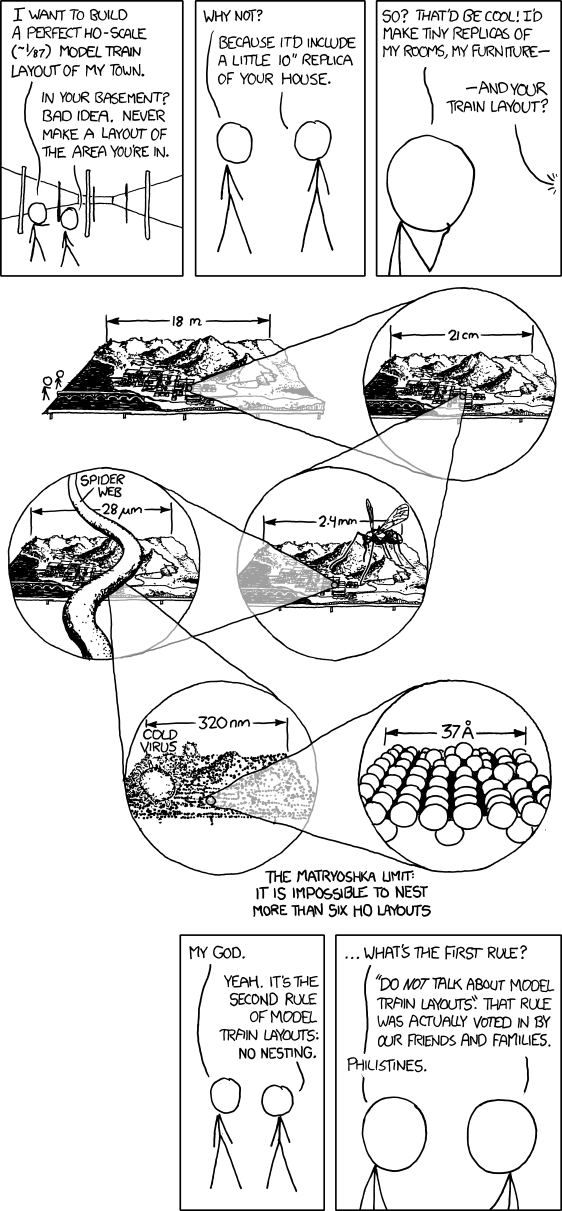
\includegraphics[width=4in]{graphics/model_rail.png}
\end{center}
\caption[xkcd 878: model rail]{\url{http://xkcd.com/878}  Math is not limited by physics, however.}
\label{fig:xkcd878}
\end{figure}
